\documentclass[compress, 13pt, aspectratio=169]{beamer}
\usepackage{siunitx}
\usepackage{physics}
\usepackage{caption}
\usepackage{graphicx}
\usepackage{mhchem}
\usepackage{siunitx}
\usepackage{subfig}
\usepackage{ragged2e}
\usepackage{xcolor}
\usepackage{amsmath}
\usepackage{hyperref}
% \usepackage[style=phys, backend=biber, articletitle=false, pageranges=false, citestyle=authoryear]{biblatex}
\usepackage[natbib=true, style=phys, autocite=footnote, articletitle=false, pageranges=false, citestyle=authoryear]{biblatex}
\usepackage{perpage} %the perpage package
\usefonttheme[onlymath]{serif}
\MakePerPage{footnote}
\urlstyle{sf}

% \bibliography{references.bib}
% \usetheme[progressbar=frametitle]{metropolis}
\usetheme{Madrid}
\usecolortheme{default}
\graphicspath{{figures/}}
\addbibresource{reference.bib}

\makeatletter
\newcommand{\srcsize}{\@setfontsize{\srcsize}{5pt}{5pt}}
\makeatother
\setbeamerfont{footnote}{size=\srcsize}
% \renewcommand\footnoterule{}
% \renewcommand{\thempfootnote}{\arabic{footnote}}
% \usepackage[warnundef]{jabbrv}
% \DefineJournalAbbreviation{Test}{Tes}
% \AtEveryCitekey{\iffootnote{\color{red}\scriptsize}{\color{blue}}}
% \DefineJournalAbbreviation{Nuclear Instruments and Methods in Physics Research Section A: Accelerators, Spectrometers, Detectors and Associated Equipment}{Nucl. Instrum. Methods Phys. Res. A}
% \DefineJournalAbbreviation{Instruments}{Instrum.}
% \DefineJournalAbbreviation{Spectrometers,}{Spectro.}



\title[Simulation Framework for the Digitization Module of Scintillators]{Simulation framework for the digitization module of scintillators and its implementation in NeuLAND}
\author[Yanzhao Wang]{Yanzhao Wang, Jan Mayer, Igor Gasparic, and Andreas Zilges}
\institute[University of Cologne $\vert$ AG Zilges $\vert$ ]{Institute for Nuclear Physics, University of Cologne}
\date{\scriptsize R3B Conference\\Budapest 2023}
\setbeamertemplate{blocks}[rounded][shadow]
\setbeamercolor{footlinecolor1}{fg=white,bg=black}
\setbeamercolor{footlinecolor2}{fg=black,bg=lightgray}
\setbeamertemplate{navigation symbols}{}
% \setbeamertemplate{frametitle}[default][center]

\setbeamertemplate{frametitle}{%
    \vspace{-0.13cm}
\begin{beamercolorbox}[wd=\paperwidth, ht=0.5cm, dp=0.2cm]{frametitle}
\center\usebeamerfont{frametitle}\insertframetitle
\end{beamercolorbox}
}

\renewbibmacro*{name:andothers}{% Based on name:andothers from biblatex.def
  \ifboolexpr{
    test {\ifnumequal{\value{listcount}}{\value{liststop}}}
    and
    test \ifmorenames
  }
    {\ifnumgreater{\value{liststop}}{1}
       {\finalandcomma}
       {}%
     \andothersdelim\bibstring[\emph]{andothers}}
    {}
}

\makeatletter
\setbeamertemplate{footline}
{
  \leavevmode%
  \hbox{%
  \begin{beamercolorbox}[wd=.5\paperwidth,ht=2.25ex,dp=1ex,center]{footlinecolor1}%
    \usebeamerfont{author in head/foot}\insertshortinstitute\insertshortauthor
  \end{beamercolorbox}%
  \begin{beamercolorbox}[wd=.5\paperwidth,ht=2.25ex,dp=1ex,center]{footlinecolor2}%
    \usebeamerfont{title in head/foot}\insertshorttitle\hspace*{2ex}
 \insertframenumber{} / \inserttotalframenumber\hspace*{2ex}
  \end{beamercolorbox}}%
  \vskip0pt%
}
\makeatother
% \setbeamercolor{block body alerted}{bg=alerted text.fg!10}
% \setbeamercolor{block title alerted}{bg=alerted text.fg!20}
% \setbeamercolor{block body}{bg=structure!10}
% \setbeamercolor{block title}{bg=structure!20}
% \setbeamercolor{block body example}{bg=green!10}
% \setbeamercolor{block title example}{bg=green!20}
\begin{document}
{
    \usebackgroundtemplate{
\includegraphics[width=\paperwidth]{TitleLogo}}
    \begin{frame}
        \titlepage
        \flushright\vspace*{2em}{\tiny Email: \textit{ywang@ikp.uni-koeln.de}}
    \end{frame}
}

{
    \usebackgroundtemplate{%
    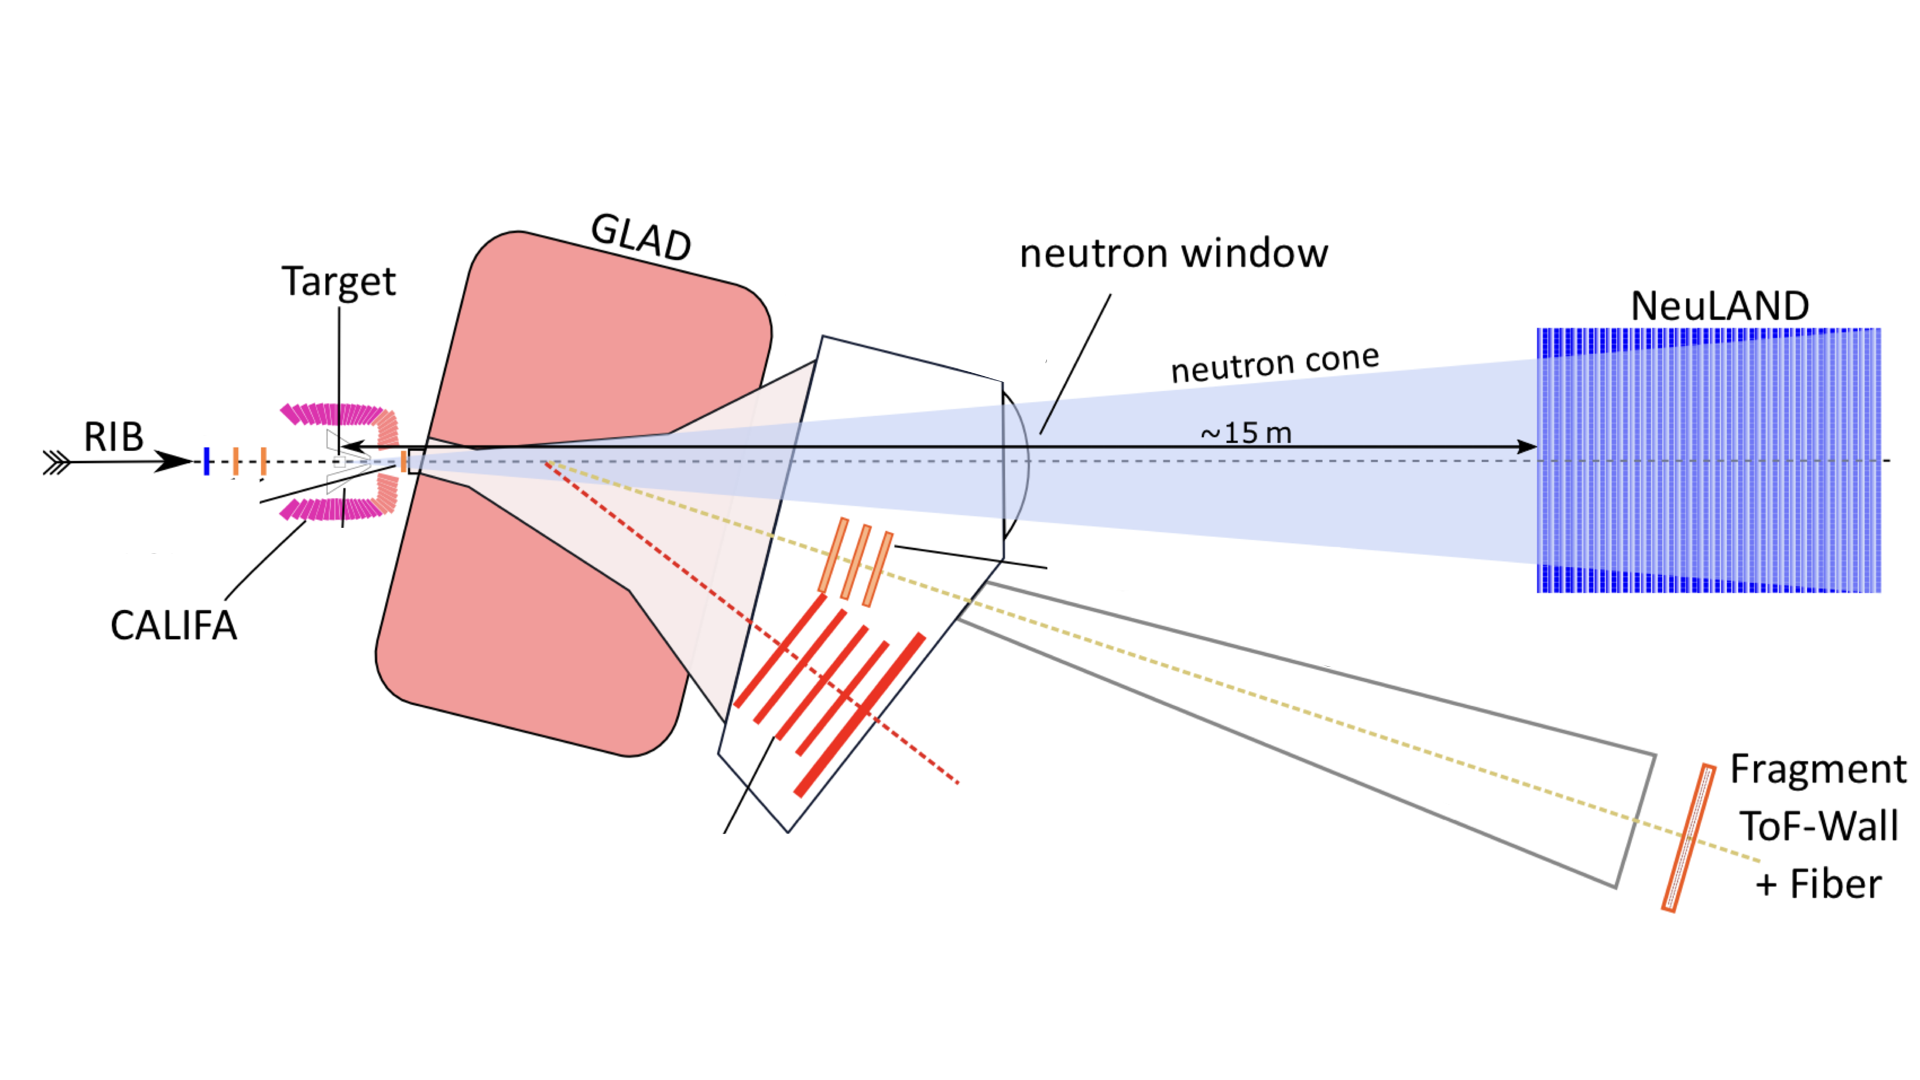
\includegraphics[width=\paperwidth, height=\paperheight]{r3bsetup_empty.png}}
    \begin{frame}{NeuLAND setup in $\text{R}^3\text{B}$}
        \begin{columns}[c]
            \begin{column}{0.4\textwidth}
                \pause
                \begin{figure}
                    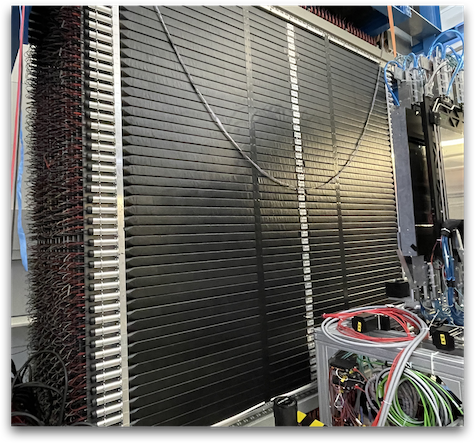
\includegraphics[width = \textwidth]{neulandReal}
                \end{figure}
            \end{column}
            \hspace*{0.5cm}
            \begin{column}{0.3\textwidth}
                \begin{exampleblock}{}
                    Geometry:\\
                    \begin{itemize}
                        \item 26 planes
                        \item $\qtyproduct[product-units=power]{250 x 250}{\centi\meter}$ 
                        \item 50 scintillation bars each plane
                        \item 100 PMTs each plane
                    \end{itemize}
                    \pause
                    Measurement:\\
                    \begin{itemize}
                        \item neutron 4-momentum
                        \item neutron multiplicity 
                    \end{itemize}
                \end{exampleblock}
            \end{column}
            \begin{column}{0.3\textwidth}
            \end{column}
        \end{columns}
        \let\thefootnote\relax\footnotetext{\fullcite{BORETZKY2021165701}}
    \end{frame}
}

\begin{frame}[t]{Why do we need a simulation?}
    \begin{columns}[t]
        \begin{column}{0.5\textwidth}
            % Method 1: Clustering \footfullcite{Neuland::TDR}
            Method 1: Clustering \footnotemark
            \begin{figure}
                \hspace*{-1cm}
                    \centering
                    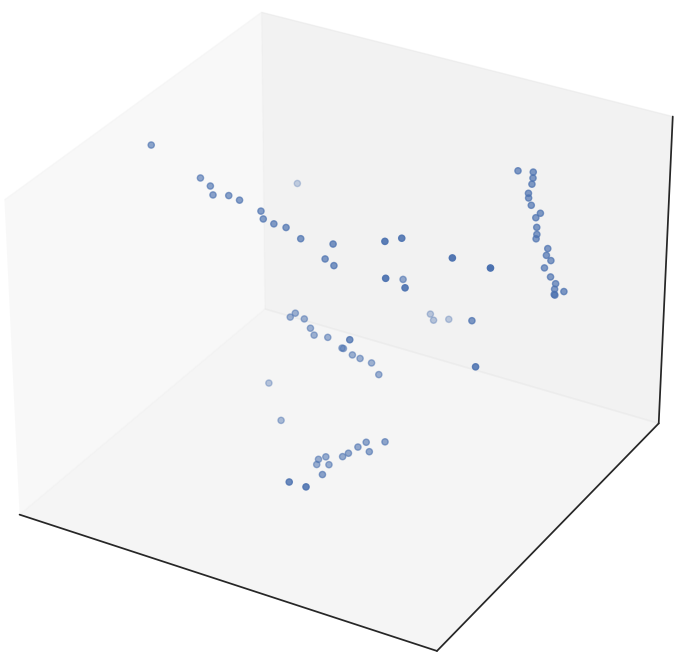
\includegraphics[width = 0.35\textwidth]{Cluster}
                    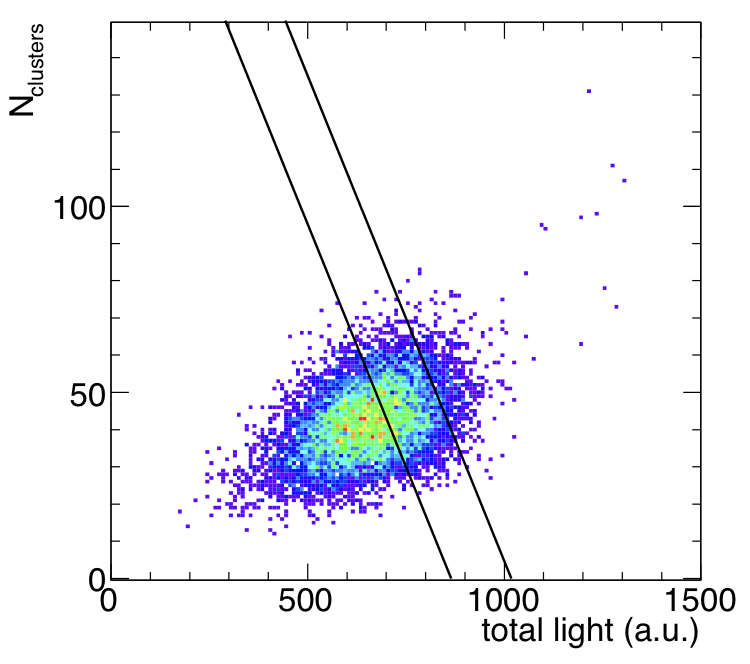
\includegraphics[width = 0.35\textwidth]{clusterPlot}
            \end{figure}
                % \vspace*{-0.2cm}
            Method 2: Bayes WCP
            $$P(H|\va{E}) = P(H) \frac{P(\va{E}|H)}{\sum_h{P(\va{E}|H_h)P(H_h)}}$$
            Method 3: Convolutional neural network 
            % \begin{figure}
            %     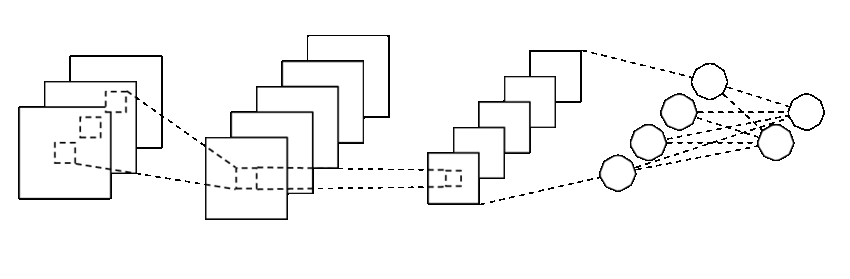
\includegraphics[width = 0.5\textwidth]{CNN}
            % \end{figure}
        \end{column}
        \begin{column}{0.5\textwidth}
            {\color{red} \onslide<2->{ \textbf{\textit{Validation?}}} \onslide<3-> {\textbf{\textit{Simulation!}}}}
            \begin{figure}[t]
                \includegraphics<1>[width = \textwidth]{FlowSimu/FlowSimu.001.png}%
                \includegraphics<2>[width = \textwidth]{FlowSimu/FlowSimu.001.png}%
                \includegraphics<3>[width = \textwidth]{FlowSimu/FlowSimu.002.png}%
                \includegraphics<4>[width = \textwidth]{FlowSimu/FlowSimu.003.png}%
                \includegraphics<5>[width = \textwidth]{FlowSimu/FlowSimu.004.png}%
            \end{figure}
            % \vspace*{-1.8cm}
            % \footnotetext[1]{\textcite{Neuland::TDR}}
        \end{column}
    \end{columns}
    \vspace*{-1.8cm}
    \footcitetext{Neuland::TDR}
\end{frame}

\begin{frame}{Digitization process}
    \begin{columns}
        \begin{column}{0.5\textwidth}
            \begin{figure}[t]
                \includegraphics<1>[keepaspectratio, height = 0.8\textheight]{digiFlow/digiFlow.001.png}%
                \includegraphics<2>[keepaspectratio, height = 0.8\textheight]{digiFlow/digiFlow.002.png}%
                \includegraphics<3>[keepaspectratio, height = 0.8\textheight]{digiFlow/digiFlow.003.png}%
                % \includegraphics<4>[keepaspectratio, height = 0.8\textheight]{digiFlow/digiFlow.004.png}%
                \includegraphics<4>[keepaspectratio, height = 0.8\textheight]{digiFlow/digiFlow.005.png}%
                \includegraphics<5>[keepaspectratio, height = 0.8\textheight]{digiFlow/digiFlow.005.png}%
                % \includegraphics<6>[keepaspectratio, height = 0.8\textheight]{digiFlow/digiFlow.005.png}%
            \end{figure}
        \end{column}
        \begin{column}{0.5\textwidth}
            \vspace*{-0.5cm}
            \begin{figure}[t]
                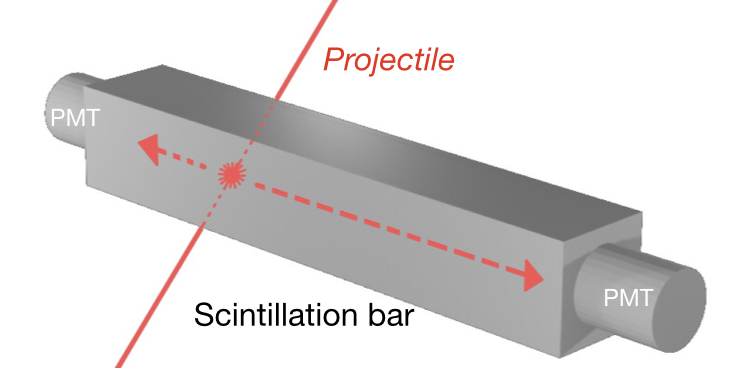
\includegraphics[keepaspectratio, height = 0.3\textheight]{Bar}%
            \end{figure}
            \vspace*{-0.5cm}
            \visible<5>
            {
            \begin{figure}[t]
                % \centering{\small Energy depositions of different Particles}
                % 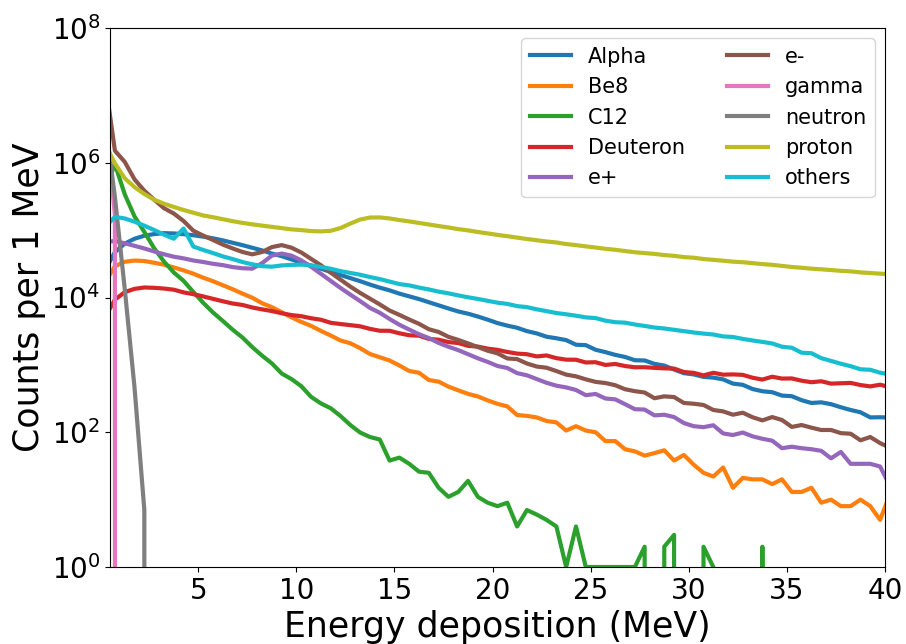
\includegraphics[keepaspectratio, height = 0.5\textheight]{Edep}%
                \centering{\small Energy depositions of different particles \tiny($E_n = \SI{600}{\mega\electronvolt}$)}
                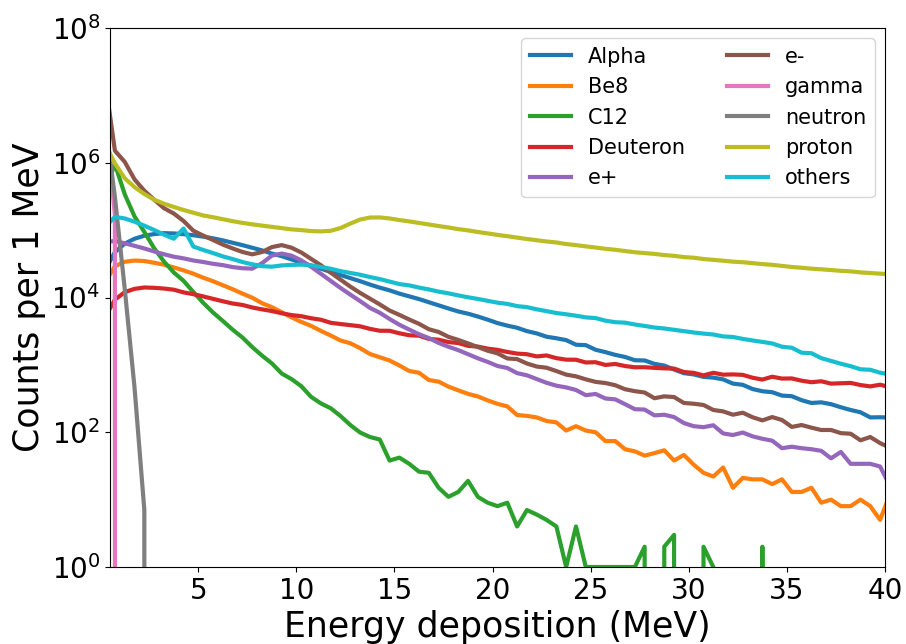
\includegraphics[keepaspectratio, height = 0.5\textheight]{Edep}%
            \end{figure}
        }
        \end{column}
    \end{columns}
\end{frame}

\begin{frame}{Simulation of scintillation bar}
    \begin{columns}
        \begin{column}{0.5\textwidth}
            \begin{figure}[t]
                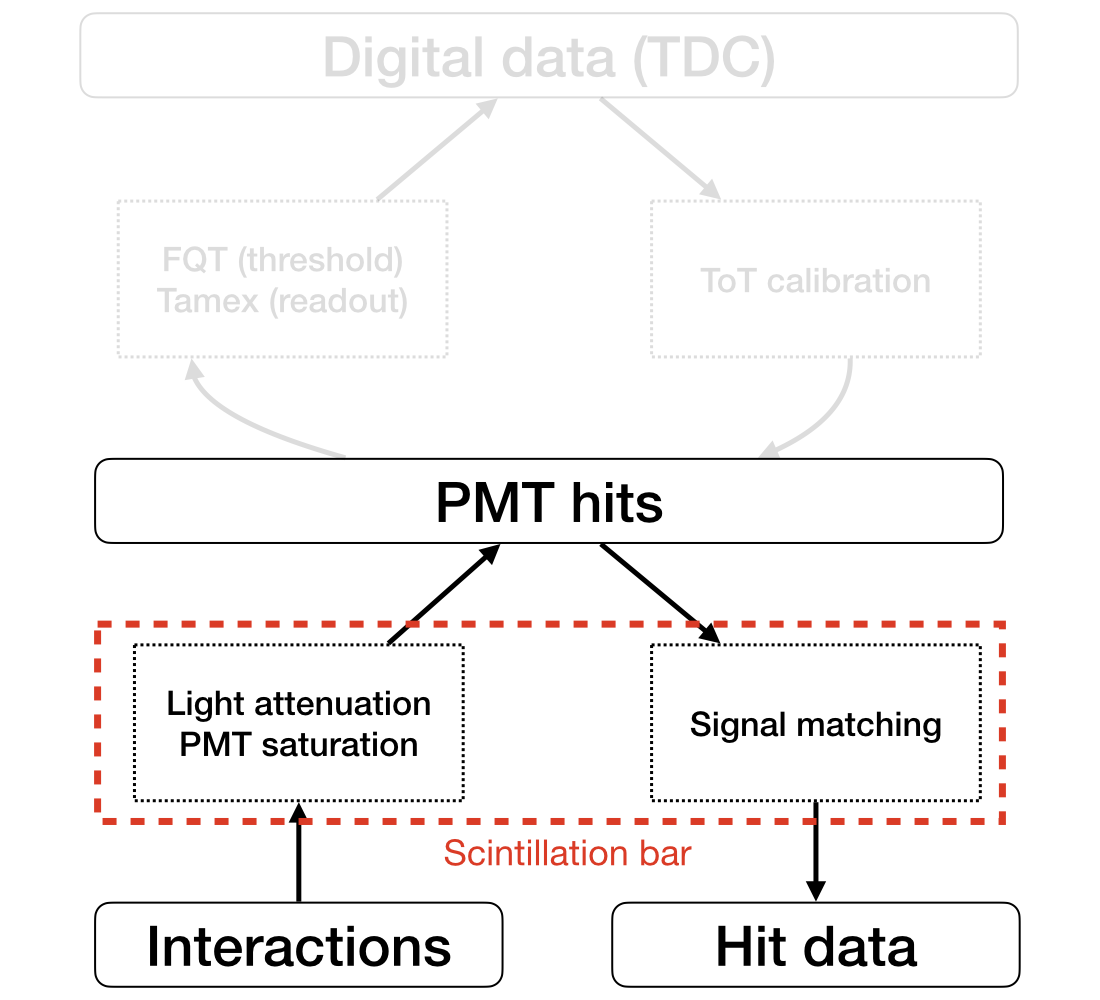
\includegraphics[keepaspectratio, height = 0.8\textheight]{digiFlow/digiFlow.006.png}%
            \end{figure}
        \end{column}
        \begin{column}{0.5\textwidth}
            % \setbeamercolor{block title}{#3}
            \setbeamercolor{block body}{bg=white, fg=black}
            \pause
            % \vspace*{-0.1cm}
            % \begin{beamercolorbox}[rounded=true, ht=1.1ex]{block title}
            %     \small PMT saturation\footnotemark 
            % \end{beamercolorbox}
            \vspace*{-0.3cm}
            \begin{block}{\small PMT saturation\footnotemark}
                \begin{figure}[t]
                    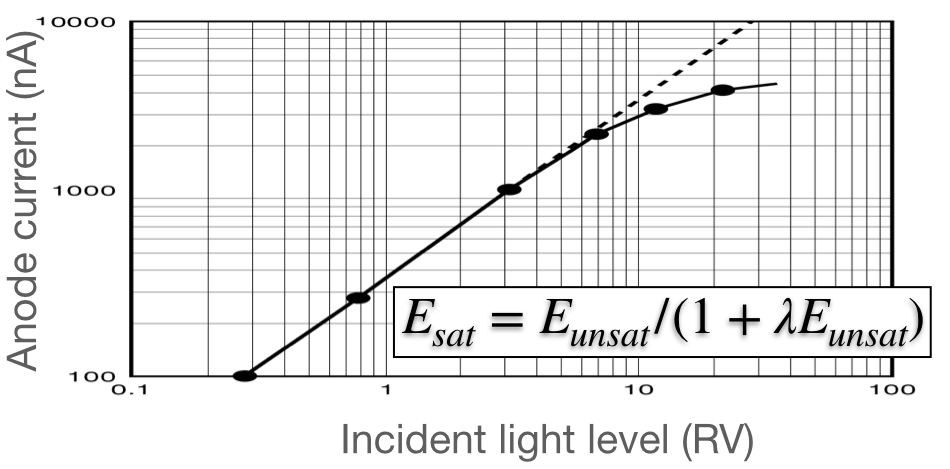
\includegraphics[keepaspectratio, height = 0.4\textwidth]{PMTSAT}%
                \end{figure}
            \end{block}
            \pause
            \vspace*{-0.2cm}
            \begin{block}{\small Light attenuation}
            \vspace*{-0.2cm}
            {
                \small$$Y_{PMT} = Y_{edep} \exp (-\alpha \cdot L)$$
            }
            \vspace*{-0.7cm}\\
            {\footnotesize$\alpha$: Attenuation factor}
            \end{block}
            \pause
            \vspace*{-0.2cm}
            \begin{block}{\small PMT signal matching}
            {
                \small
                \vspace*{-0.5cm}
                $$\text{min }\Delta = 
                \begin{cases}
                    \lvert E_1/E_2 \cdot e^{\alpha c (t_1-t_2)} -1\rvert\ ,& t_1>t_2\\
                    \lvert E_2/E_1 \cdot e^{\alpha c (t_2-t_1)} -1\rvert\ ,& t_2>t_1\\
                \end{cases}$$
            }
            \end{block}
        \end{column}
    \end{columns}
    % \footcitetext{Hamamatsu}
    \footnotetext{\fullcite{Hamamatsu}}
\end{frame}

\begin{frame}{Simulation of digitization channel}
    \begin{columns}
        \begin{column}{0.5\textwidth}
            \begin{figure}[t]
                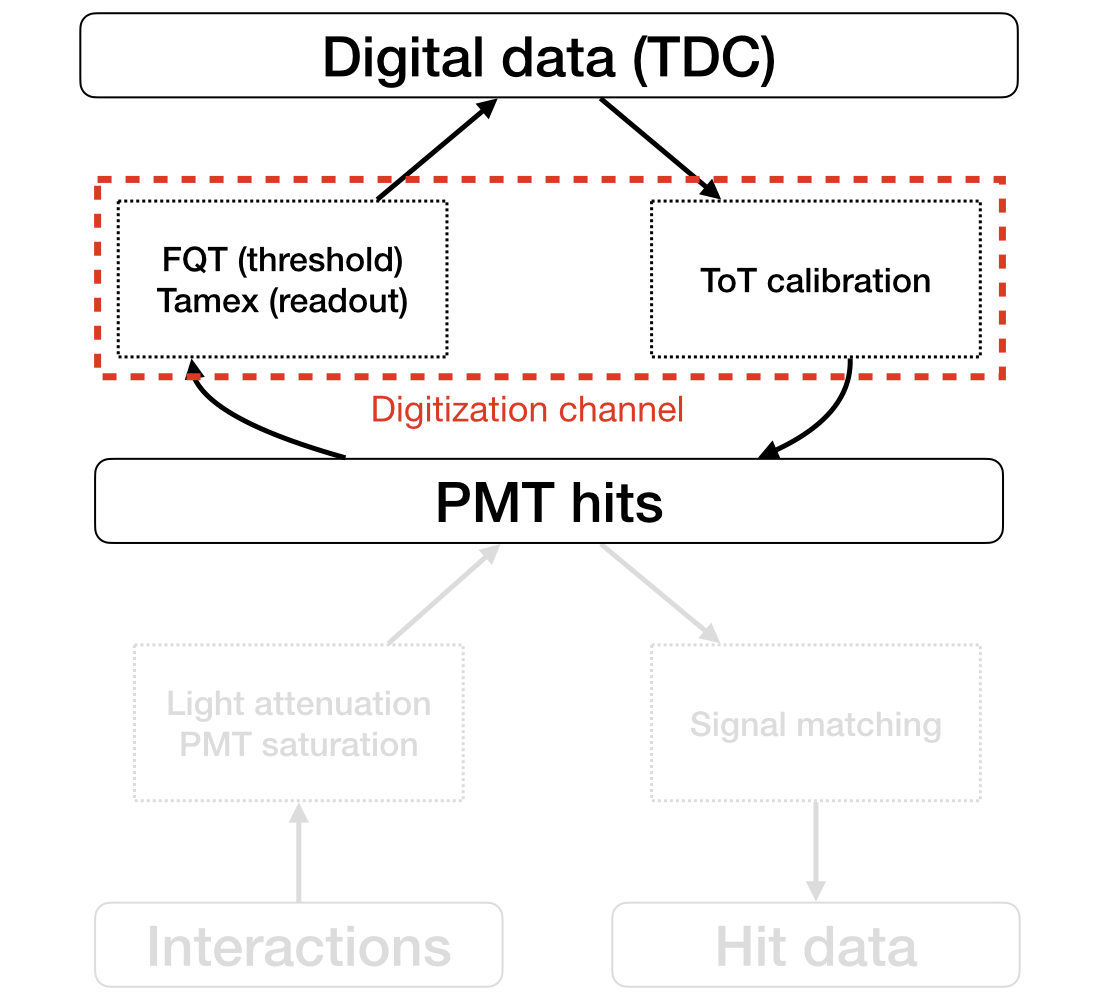
\includegraphics[keepaspectratio, height = 0.8\textheight]{digiFlow/digiFlow.007.png}%
            \end{figure}
        \end{column}
        \begin{column}{0.5\textwidth}
            \begin{figure}[t]
                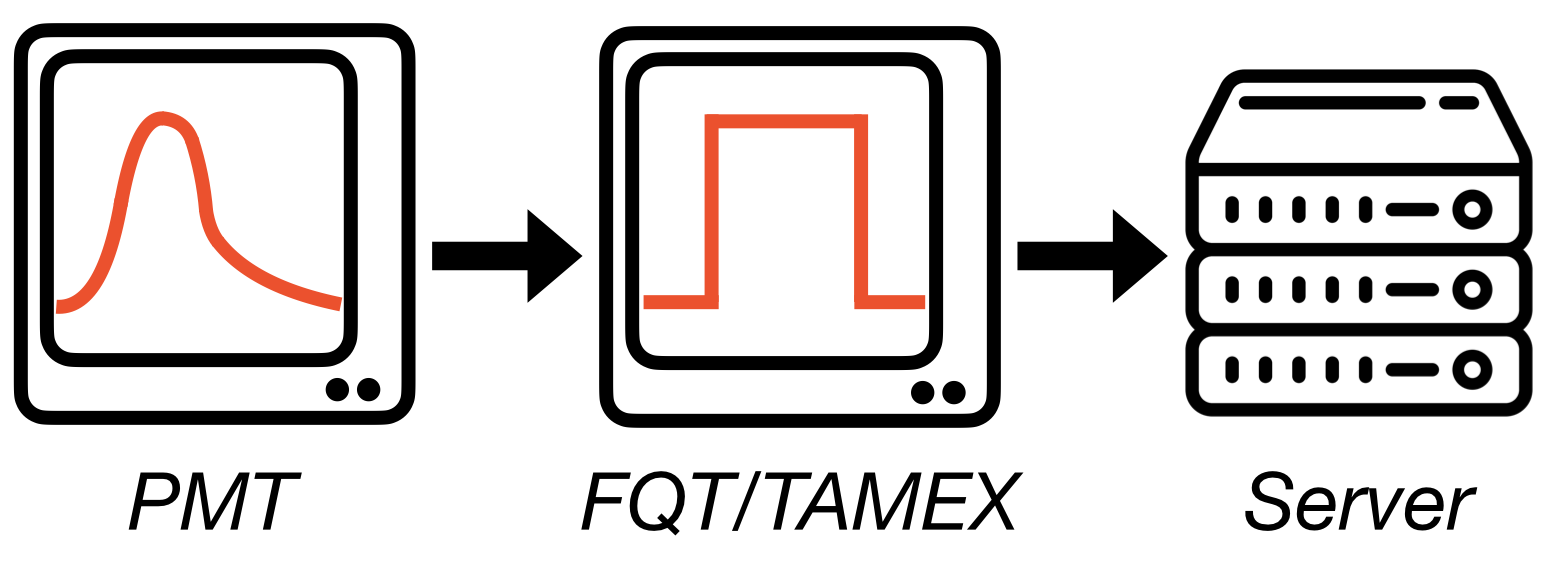
\includegraphics[keepaspectratio, height = 0.3\textwidth]{PMT2TAMEX.png}%
            \end{figure}
            \pause
            \begin{block}{Simulation steps}
                \begin{enumerate}
                        \setbeamercovered{transparent}
                    \item<2-> Apply threshold
                    \item<3-> Perform pileup of PMT signals (addition)
                    \item<3-> PMT signals $\Rightarrow$ FQT signals
                    \item<4-> Perform pileup of FQT signals (merge)
                    \item<4-> Energy and time value smearing
                \end{enumerate}
            \end{block}
        \end{column}
    \end{columns}
\end{frame}

\begin{frame}{Total energy deposition}
    \vspace*{-0.7cm}
    \begin{columns}
        \begin{column}{0.5\textwidth}
            \begin{figure}[t]
                \centering{\small Neutron multiplicity = 4}
                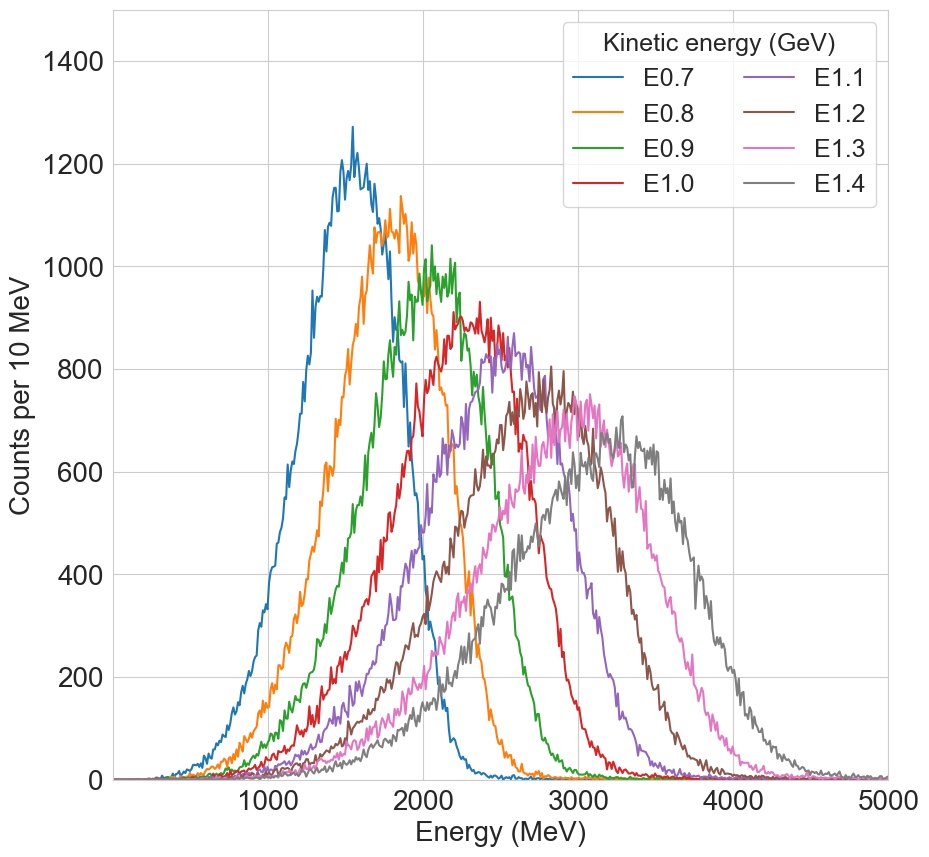
\includegraphics[keepaspectratio, width = \textwidth]{Plots/ETot_4n}%
            \end{figure}
        \end{column}
        \begin{column}{0.5\textwidth}
            \begin{figure}[t]
                \centering{\small Neutron kinetic energy = $\SI{1}{\giga\electronvolt}$}
                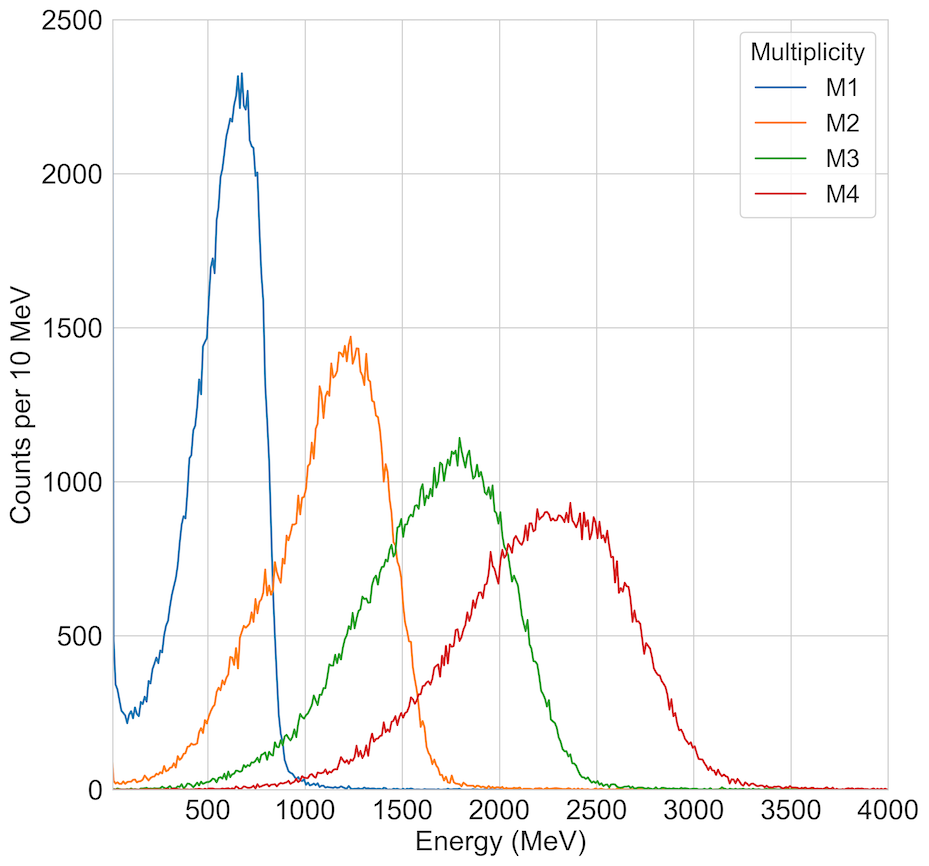
\includegraphics[keepaspectratio, width = \textwidth]{Plots/ETot_E1}%
            \end{figure}
        \end{column}
    \end{columns}
\end{frame}


\begin{frame}{Energy deposition of hits}
    \vspace*{-0.6cm}
    \begin{columns}
        \begin{column}{0.5\textwidth}
            \begin{figure}[t]
                \centering{\small Neutron multiplicity = 4}
                \includegraphics[keepaspectratio, width = 0.9\textwidth]{Plots/Ehit_4n}%
            \end{figure}
        \end{column}
        \begin{column}{0.5\textwidth}
            \begin{figure}[t]
                \centering{\small Neutron kinetic energy = $\SI{1}{\giga\electronvolt}$}
                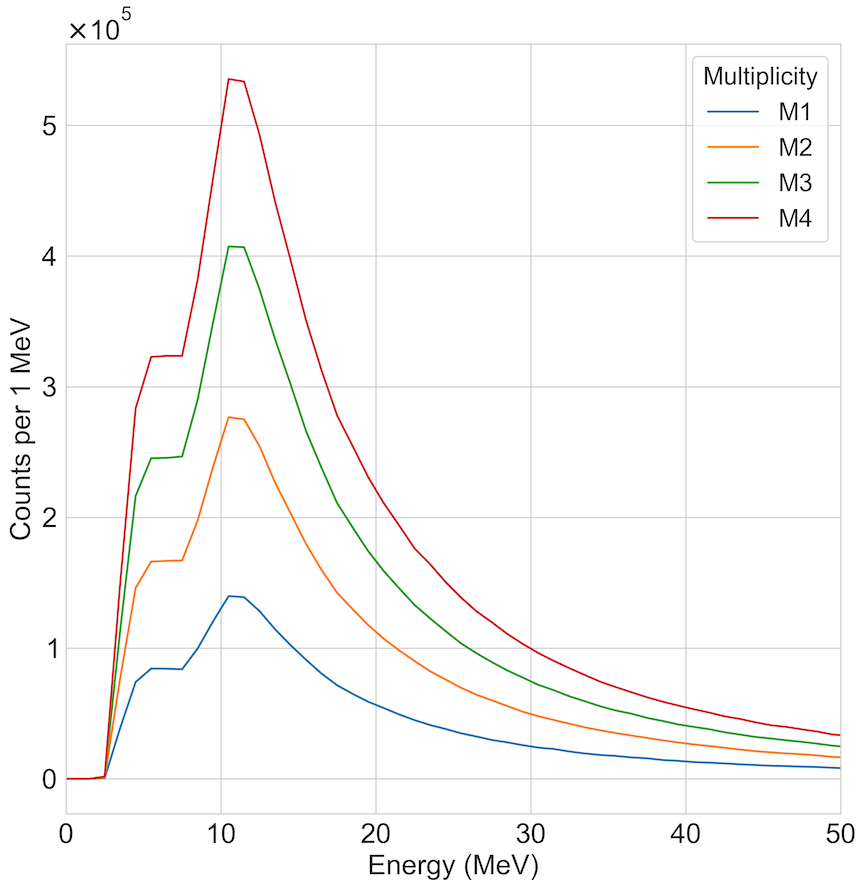
\includegraphics[keepaspectratio, width = 0.9\textwidth]{Plots/Ehit_E1}%
            \end{figure}
        \end{column}
    \end{columns}
\end{frame}

\begin{frame}{Comparisons to Tacquila and mockup}
    \vspace*{-0.6cm}
    \begin{columns}
        \begin{column}{0.5\textwidth}
            \begin{figure}[t]
                \centering{\small Hit energy deposition ($M=4, KE=\SI{1}{\giga\electronvolt}$)}
                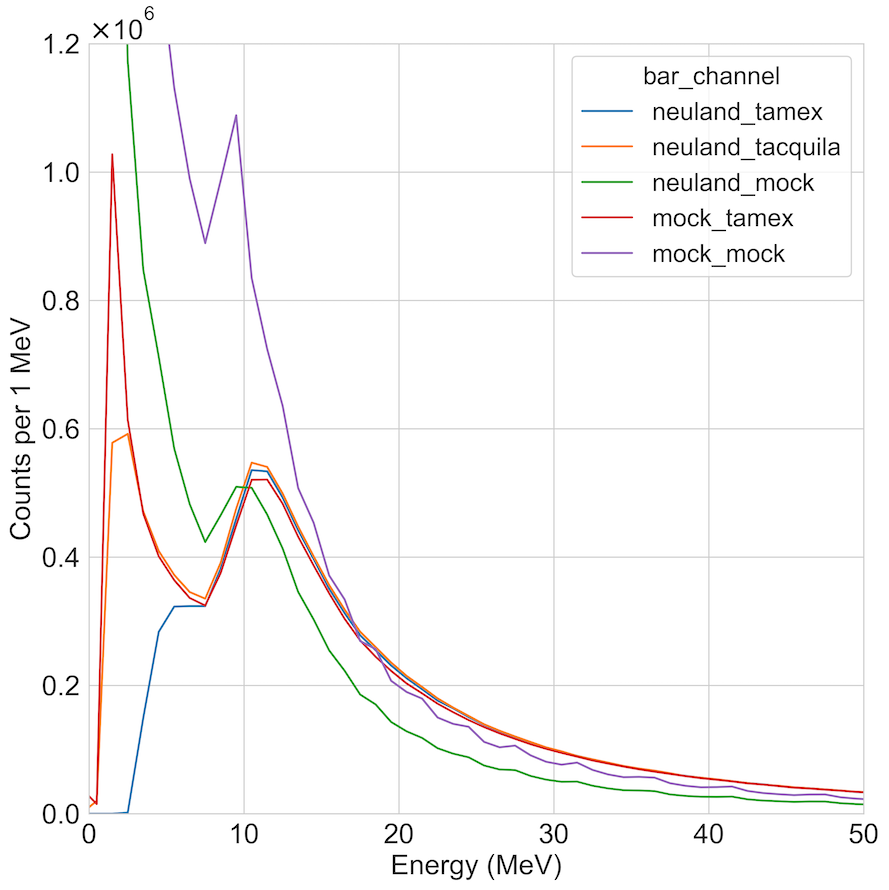
\includegraphics[keepaspectratio, width = 0.9\textwidth]{Plots/EHitAll_E1_4n.png}%
            \end{figure}
        \end{column}
        \begin{column}{0.5\textwidth}
            \begin{figure}[t]
                \centering{\small Total energy deposition ($M=4, KE=\SI{1}{\giga\electronvolt}$)}
                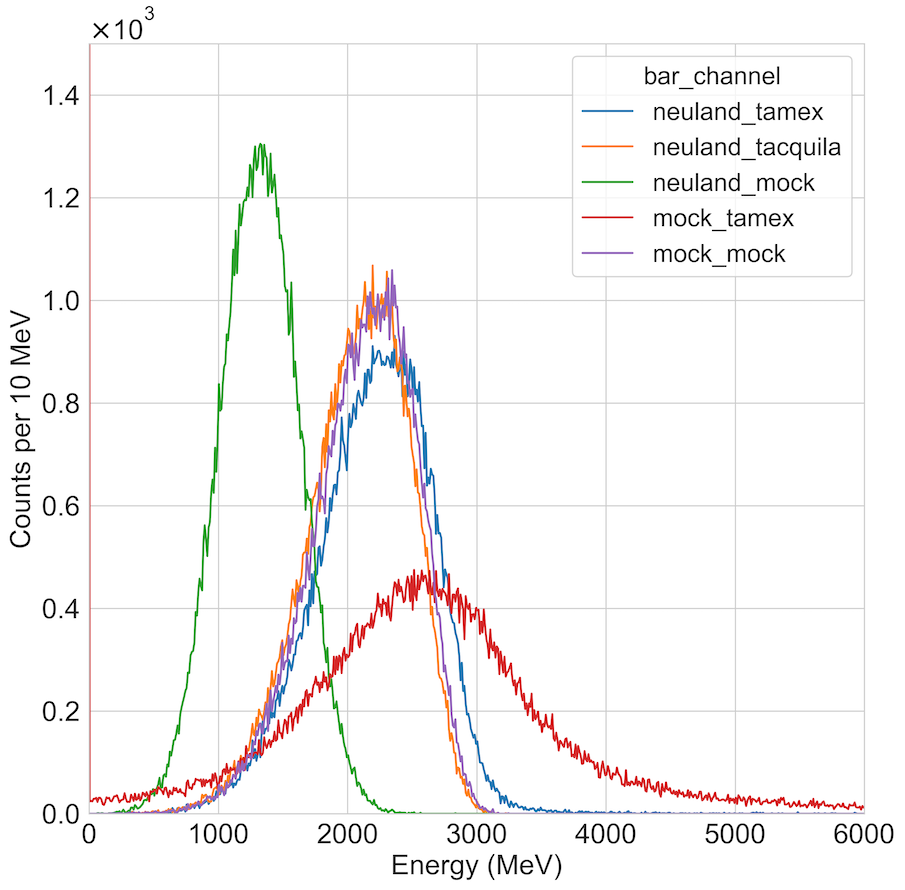
\includegraphics[keepaspectratio, width = 0.9\textwidth]{Plots/EtotAll_E1_4n.png}%
            \end{figure}
        \end{column}
    \end{columns}
\end{frame}

\begin{frame}{Summary and outlook}
    \begin{columns}
        \begin{column}{0.5\textwidth}
            \begin{block}{In this talk}
                \begin{itemize}
                    \item simulation on scintillation bars and digitization channels
                    \item multi-hit capability
                    \item distribution on total energy deposition and hit energies
                    \item better performance on low energy filtering
                \end{itemize}
            \end{block}

            \begin{exampleblock}{What to do next}
                \begin{itemize}
                    \item integration time window on Tamex
                    \item comparison to real calibrated data
                    \item applications on other detectors
                \end{itemize}
            \end{exampleblock}
        \end{column}
        \begin{column}{0.5\textwidth}
            \begin{figure}[t]
                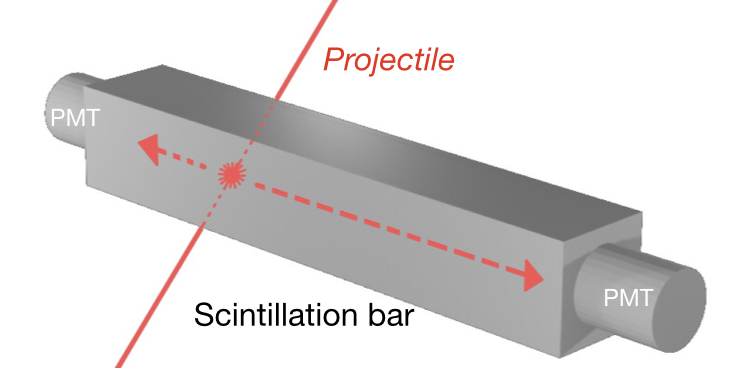
\includegraphics[keepaspectratio, width = 0.4\textwidth]{Bar}%
                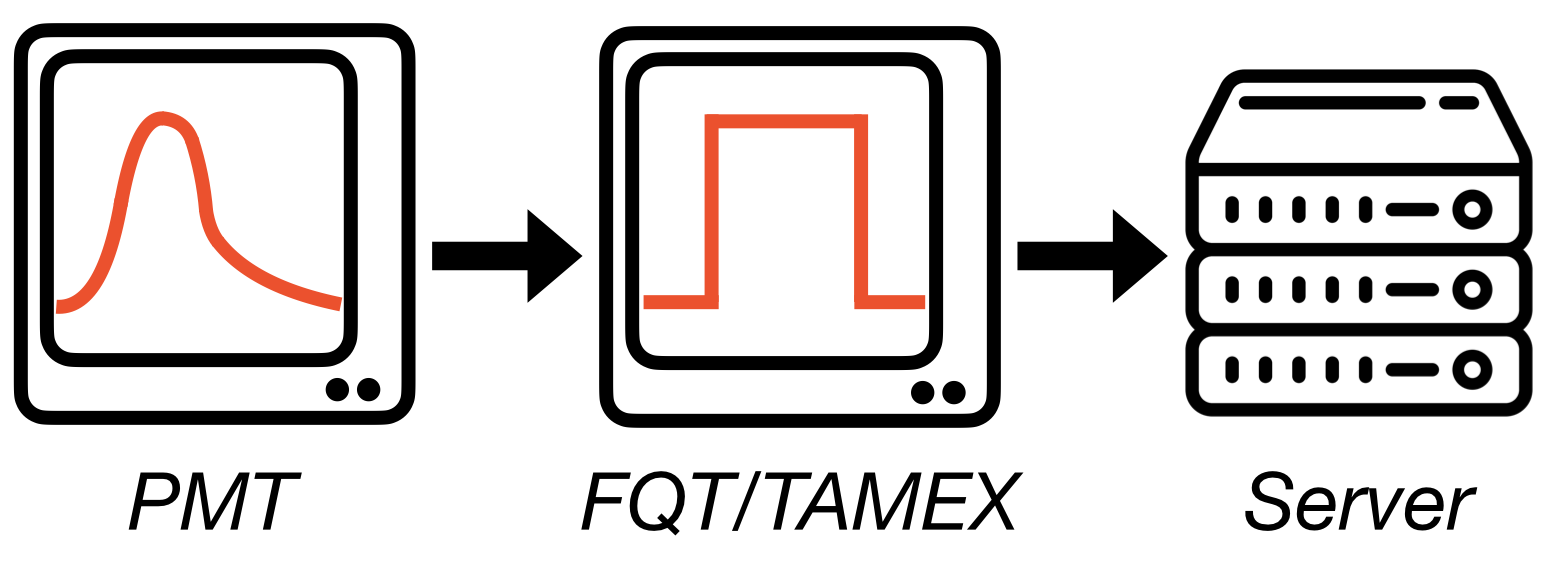
\includegraphics[keepaspectratio, width = 0.4\textwidth]{PMT2TAMEX.png}%
            \end{figure}
            \begin{figure}[t]
                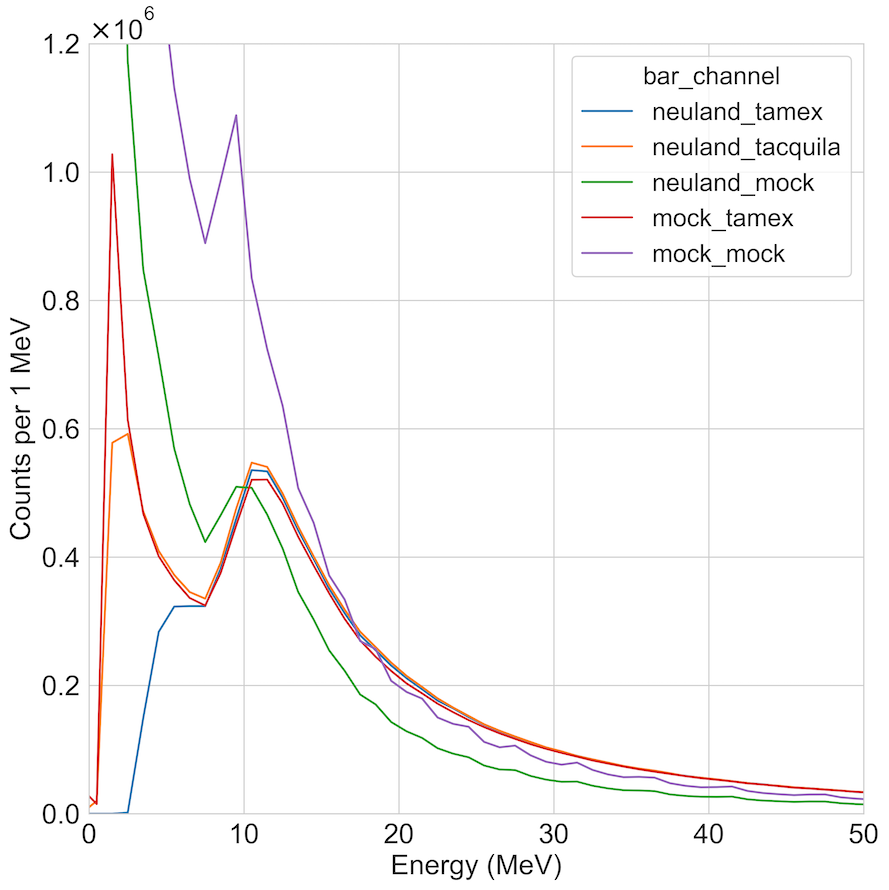
\includegraphics[keepaspectratio, width = 0.6\textwidth]{Plots/EHitAll_E1_4n.png}%
            \end{figure}
        \end{column}
    \end{columns}
\end{frame}
    
% \end{Summary and outlook}
% % \begin{columns}
% %     \begin{column}{0.5\textwidth}
% %     \end{column}
% %     \begin{column}{0.5\textwidth}
% %     \end{column}
% % \end{columns}
\end{document}

